\section{Panorama Atual sobre EPT no Brasil} 


Neste capítulo apresentamos um panorama nacional sobre as matrículas por tipos de dependência Estadual, Federal, Municipal e Privada (incluído o Sistema S).  Fica evidenciado que o Brasil possui quatro redes robustas que lideram as ofertas, variando sua participação dependendo de cada Estado. No simulador interativo na internet é possível acessar e pesquisar por  UF:
\href{https://datanalytics.worldbank.org/content/6604f317-d487-436a-b6b6-792369b341f0}{https://datanalytics.worldbank.org/Plataforma Interativo PROPAG}  



\begin{figure}[htbp!]
	\centering
	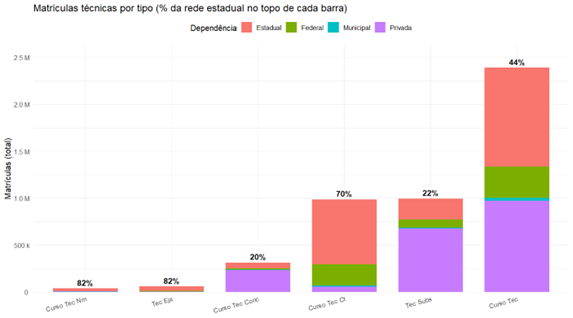
\includegraphics[width=1\textwidth]{images/3a_MaTec.png}
	\caption{Aba C: Matricula Técnicas por tipo} 
	\label{fig:3a_MaTec}
\end{figure}


Este  primeiro gráfico \ref{fig:3a_MaTec} apresenta o cenário da oferta da EPT por meio das diversas redes de ensino. As redes estaduais são as maiores ofertantes, seguidas pela oferta da rede privada (incluindo o Sistema S) e indicam uma evolução da Rede Federal com a expansão dos Institutos Federais (IFs).

O próximo gráfico  \ref{fig:3b_MaTec} na sequência apresenta uma panorâmica das Matrículas de Educação Profissional Técnica (EPT) por Unidade da Federação e a participação de cada rede. Novamente as redes estaduais e a rede privada, com variáveis por UF, lideram também o [\textcolor{red}{MARINA ou TEXTO ACABOU}]

\begin{figure}[htbp!]
	\centering
	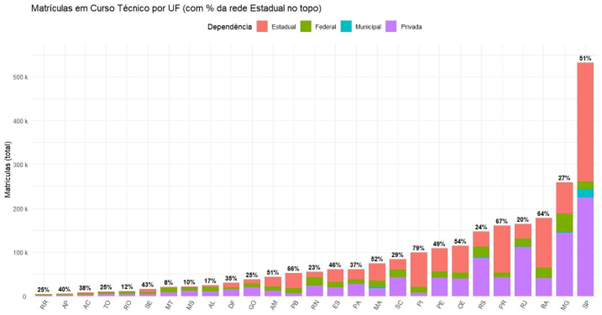
\includegraphics[width=1\textwidth]{images/3b_MaTec.png}
	\caption{Aba C: Matriculas em Curso Técnico por tipo} 
	\label{fig:3b_MaTec}
\end{figure}


\section{Política de coordenação entre redes}

Um dos desafios importantes do Programa de Expansão da EPT no Brasil e nas UFs é a coordenação e articulação das diversas redes e instituições de ensino ofertantes de cursos técnicos. É fundamental a elaboração e consolidação de uma Política Estadual de EPT em cada UF e que sejam superadas as descontinuidades de políticas, programas e projetos após cada ciclo de governo, tanto no âmbito federal como estadual. 

A EPT no Brasil já conta com uma estrutura instalada de instituições públicas e privadas de grande impacto. O país tem 29.993 escolas de ensino médio funcionando; 661 unidades (campi) vinculadas a 38 Institutos Federais (IFs), 02 Centros Federais de Educação Tecnológica (Cefet), uma Universidade Tecnológica Federal do Paraná (UTFPR), 22 escolas técnicas vinculadas às universidades federais e o Colégio Pedro II no Rio de Janeiro, além de ofertas de cursos técnicos em municípios brasileiros.

Como parceiros que já ofertam cerca de 21\% das matrículas de EPT no Brasil destacam-se as Escolas Privadas e Confessionais; o Sistema S, nome do conjunto das organizações criadas pelos setores produtivos (indústria, comércio, agricultura, transportes, cooperativas e microempresas), voltadas para qualificação profissional, pesquisa e assistências técnica e social com mais de 500 escolas em 3.431 unidades e, ainda, 2.264 Instituições Privadas de Ensino Superior (IPES).

O PROPAG apresenta uma oportunidade na perspectiva de  priorização e potencialização de todas as estruturas das diversas redes e parceiros para focar os investimentos na ampliação das matrículas e nas condições de ensino-aprendizagem dos estudantes da EPT. É uma oportunidade histórica para cada Estado e para o país formação de uma grande geração de técnicos de nível médio antes da transição demográfica estrutural em curso.